\documentclass{beamer}
\usepackage[utf8]{inputenc}

\usetheme{Madrid}
\usecolortheme{default}
\usepackage{amsmath,amssymb,amsfonts,amsthm}
\usepackage{txfonts}
\usepackage{tkz-euclide}
\usepackage{listings}
\usepackage{adjustbox}
\usepackage{array}
\usepackage{tabularx}
\usepackage{gvv}
\usepackage{lmodern}
\usepackage{circuitikz}
\usepackage{tikz}
\usepackage{graphicx}

\setbeamertemplate{page number in head/foot}[totalframenumber]

\usepackage{tcolorbox}
\tcbuselibrary{minted,breakable,xparse,skins}



\definecolor{bg}{gray}{0.95}
\DeclareTCBListing{mintedbox}{O{}m!O{}}{%
  breakable=true,
  listing engine=minted,
  listing only,
  minted language=#2,
  minted style=default,
  minted options={%
    linenos,
    gobble=0,
    breaklines=true,
    breakafter=,,
    fontsize=\small,
    numbersep=8pt,
    #1},
  boxsep=0pt,
  left skip=0pt,
  right skip=0pt,
  left=25pt,
  right=0pt,
  top=3pt,
  bottom=3pt,
  arc=5pt,
  leftrule=0pt,
  rightrule=0pt,
  bottomrule=2pt,

  colback=bg,
  colframe=orange!70,
  enhanced,
  overlay={%
    \begin{tcbclipinterior}
    \fill[orange!20!white] (frame.south west) rectangle ([xshift=20pt]frame.north west);
    \end{tcbclipinterior}},
  #3,
}
\lstset{
    language=C,
    basicstyle=\ttfamily\small,
    keywordstyle=\color{blue},
    stringstyle=\color{orange},
    commentstyle=\color{green!60!black},
    numbers=left,
    numberstyle=\tiny\color{gray},
    breaklines=true,
    showstringspaces=false,
}
%------------------------------------------------------------
%This block of code defines the information to appear in the
%Title page
\title %optional
{1.4.19}
\date{August  2025}
%\subtitle{A short story}

\author % (optional)
{Namaswi - EE25BTECH11060}



\begin{document}


\frame{\titlepage}
\begin{frame}{Question}
 Show that the points $\vec{A}(1,-2,-8)$,$\vec{B}(5,0,-2)$ and $\vec{C}(11,3,7)$ are collinear and find the ratio in which B divides AC.
 
 

\end{frame}
 
\begin{frame}{given data}
 

\[
\begin{array}{|c|c|c|c|}
\hline
\textbf{Point} & \textbf{x} & \textbf{y} & \textbf{z} \\
\hline
A & 1 & -2 & -8 \\
B & 5 & 0 & -2 \\
C & 11 & 3 & 7 \\
\hline
\end{array}
\]

   
\end{frame}

\begin{frame}{Formula}
  collinearity matrix can be expressed as 

\begin{align*}
  \brak{B-A\;\;\;C-A} =\begin{myvec}{4  & 10\\2 & 5\\6  & 15}\end{myvec}
 \end{align*}
\end{frame}
 


\begin{frame}{allowframebreaks}
\frametitle{Row reduction}

     
 

\[
\left(
\begin{array}{cc}
4 & 10 \\
2 & 5 \\
6 & 15
\end{array}
\right)
R_3 \leftarrow R_3 - (R_1 + R_2)
\;
\left(
\begin{array}{cc}
4 & 10 \\
2 & 5 \\
0 & 0
\end{array}
\right)
\quad
R_1 \leftarrow R_1 - (2R_2)
\quad
\left(
\begin{array}{cc}
0 & 0 \\
2 & 5 \\
0 & 0
\end{array}
\right)
\]
 

Which is a Rank 1 matrix , Hence   $\vec{A}(1,-2,-8)$,$\vec{B}(5,0,-2)$ and $\vec{C}(11,3,7)$ are collinear.
\end{frame}

\begin{frame}{solution}
    \frametitle{finding ratio}
    Section formula for a vector $\vec{B}$ which divides the line formed by vectors $\vec{A}$ and $\vec{C}$ in the ratio k:1 is given by

\begin{align}
    \vec{B}=\frac{k\vec{C}+\vec{A}}{k+1}\\
             \myvec{5\\0\\-2} &=\frac{{\myvec{1\\-2\\-8}+k\myvec{11\\3\\7}}}{1+k}\\
    \implies\myvec{5\\0\\-2} + k\myvec{5\\0\\-2} &=\myvec{1\\-2\\-8}+k\myvec{11\\3\\7}\\ 
    \implies \myvec{4 \\2 \\6} &= k\myvec{6 \\ 3 \\9}\\
    \implies k = \frac{2}{3}
\end{align}
\end{frame}
\begin{frame}
$k=\frac{2}{3}$\\
     $\vec{B}$ which divides  $\vec{A}\vec{C}$ in the ratio 2:3


\end{frame}






\begin{frame}[fragile]
    \frametitle{Python Code}
    \begin{lstlisting}
 # Plotting points A(1, -2, -8), B(5, 0, -2), and C(11, 3, 7)
 
import numpy as np
import matplotlib.pyplot as plt
from mpl_toolkits.mplot3d import Axes3D

# Define the points as numpy arrays
A = np.array([1, -2, -8])
B = np.array([5, 0, -2])
C = np.array([11, 3, 7])
\end{lstlisting}
\end{frame}

\begin{frame}[fragile]
    \frametitle{Python Code}

    \begin{lstlisting}
 # Create a 3D plot
fig = plt.figure(figsize=(8, 6))
ax = fig.add_subplot(111, projection='3d')

# Plot the points
ax.scatter(*A, color='red', s=100, label='A(1, -2, -8)')
ax.scatter(*B, color='green', s=100, label='B(5, 0, -2)')
ax.scatter(*C, color='blue', s=100, label='C(11, 3, 7)')



    \end{lstlisting}
\end{frame}

\begin{frame}[fragile]
    \frametitle{Python Code}

    \begin{lstlisting}
 # Plot line AC
ax.plot([A[0], C[0]], [A[1], C[1]], [A[2], C[2]], color='purple', label='Line AC')

# Annotate points
ax.text(*A, ' A', color='red', fontsize=10)
ax.text(*B, ' B', color='green', fontsize=10)
ax.text(*C, ' C', color='blue', fontsize=10)


    \end{lstlisting}
\end{frame}

\begin{frame}[fragile]
    \frametitle{Python Code}

    \begin{lstlisting}
 # Set axes labels
ax.set_xlabel('X-axis')
ax.set_ylabel('Y-axis')
ax.set_zlabel('Z-axis')
ax.set_title('3D Plot of Points A, B, C and Line AC')
ax.legend()
ax.grid(True)

# Show the plot
plt.show()



\end{lstlisting}
\end{frame}

 



 


\begin{frame}[fragile]
\frametitle{C Code}
\begin{lstlisting}
  
#include <stdio.h>

int main(){
    double Ax = 1, Ay = -2, Az = -8;
    double Bx = 5, By = 0, Bz = -2;
    double Cx = 11, Cy = 3, Cz = 7;

    double kx = (Bx - Ax) / (Cx - Bx);
    double ky = (By - Ay) / (Cy - By);
    double kz = (Bz - Az) / (Cz - Bz);

    printf("%lf",kx);

    return 0;

}





\end{lstlisting}

\end{frame}


\begin{frame}[fragile]
\frametitle{Python and C Code}

\begin{lstlisting}
 import subprocess

# Compile the C program
subprocess.run(["gcc", "points.c", "-o", "points"])

# Run the compiled C program
result = subprocess.run(["./points"], capture_output=True, text=True)

# Print the output from the C program (solution steps for k=2/3)
print(result.stdout) 

\end{lstlisting}

\end{frame}

 


\begin{figure}
    \centering
    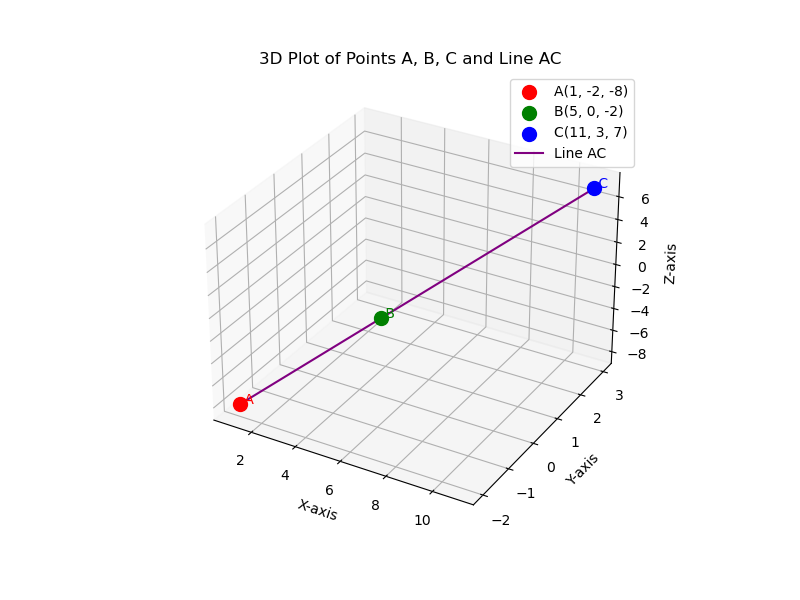
\includegraphics[width=0.8\columnwidth]{Fig.png}
    \caption{Plot}
    \label{fig:placeholder}
\end{figure}


\end{document}